\documentclass{standalone}
\usepackage{tikz}
\usetikzlibrary{calc,patterns,decorations.pathmorphing,decorations.markings}

\begin{document}

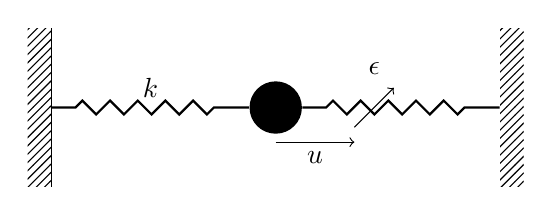
\begin{tikzpicture}
\tikzstyle{spring}=[thick,decorate,decoration={zigzag,pre length=0.3cm,post length=0.3cm,segment length=10}]
\tikzstyle{damper}=[thick,decoration={markings,  
  mark connection node=dmp,
  mark=at position 0.5 with 
  {
    \node (dmp) [thick,inner sep=0pt,transform shape,rotate=-90,minimum width=15pt,minimum height=3pt,draw=none] {};
    \draw [thick] ($(dmp.north east)+(2pt,0)$) -- (dmp.south east) -- (dmp.south west) -- ($(dmp.north west)+(2pt,0)$);
    \draw [thick] ($(dmp.north)+(0,-5pt)$) -- ($(dmp.north)+(0,5pt)$);
  }
}, decorate]
\tikzstyle{ground}=[fill,pattern=north east lines,draw=none,minimum width=0.75cm,minimum height=0.3cm]

% ========= bucks
\node (wall) [ground, rotate=-90, minimum width=2cm] {};
\draw (wall.north east) -- (wall.north west);

\node (mass2) [circle,fill] at(3,0) {$m$};

\node (wall2) at(6,0) [ground, rotate=90, minimum width=2cm] {};
\draw (wall.north east) -- (wall.north west);
% ====== connections
\draw [spring] (wall) -- node [above] {$k$} (mass2);
\draw [spring] (mass2) -- (wall2);
%% ===== comments
\draw [->] (mass2.south) ++ (0,-.1) -- node [below] {$u$} +(1,0);
\draw [->] (4,-.25) -- (4.5,.25);
\node at (4.25,.5) {$\epsilon$};
\end{tikzpicture}

\end{document}